\section{Methods}

In this section, we will describe our preliminary work parallelizing DNACLUST to work with the ever-increasing amount of sequencing data produced by today's sequencing technologies.
Then, we will propose a new clustering tool that uses an efficient $k$-difference string matching algorithm.
Finally, we will discuss how to improve the quality of each cluster by handling the alignment of ambiguous reads, an issue largely ignored by existing clustering tools.

\subsection{Parallelizing sequence recruitment to a cluster center}

Due to the large scale of sequencing data produced, clustering tools must utilize multiple processors to process the data in a timely manner.  Only half the tools presented in Table \ref{table:clustering_tools} are capable of multi-core support. Fast clustering tools such as CD-HIT and UCLUST already implement support for multiple threads.
Here, we present two parallel approaches for recruiting sequences to a cluster center within DNACLUST.
The first approach (na{\"i}ve) is based on evenly partitioning the sequences among the processors.
The second approach (work-based) involves partitioning the sequences based on the potential work that needs to be done when calculating the edit distance to the center.
If the sequences are stored in a trie-like data structure, then it is beneficial to partition highly similar sequences together despite potentially assigning an uneven number of sequences to each processor.
We implement these parallel approaches in DNACLUST show the speed-ups when clustering tens of millions of 16S rRNA sequences.

\subsubsection{Na{\"i}ve parallelization strategy}

The second step of DNACLUST's algorithm involves recruiting all sequences that lie within a given distance of the current cluster center.
Given $p$ processors, we can evenly partition the database into $p$ chunks such that each processor can calculate the edit distance independently in parallel.
We have added pthread support to the DNACLUST code, allowing us to assign a contiguous chunk of the sequence database to each thread.

\begin{figure}[tb]
  \centering
    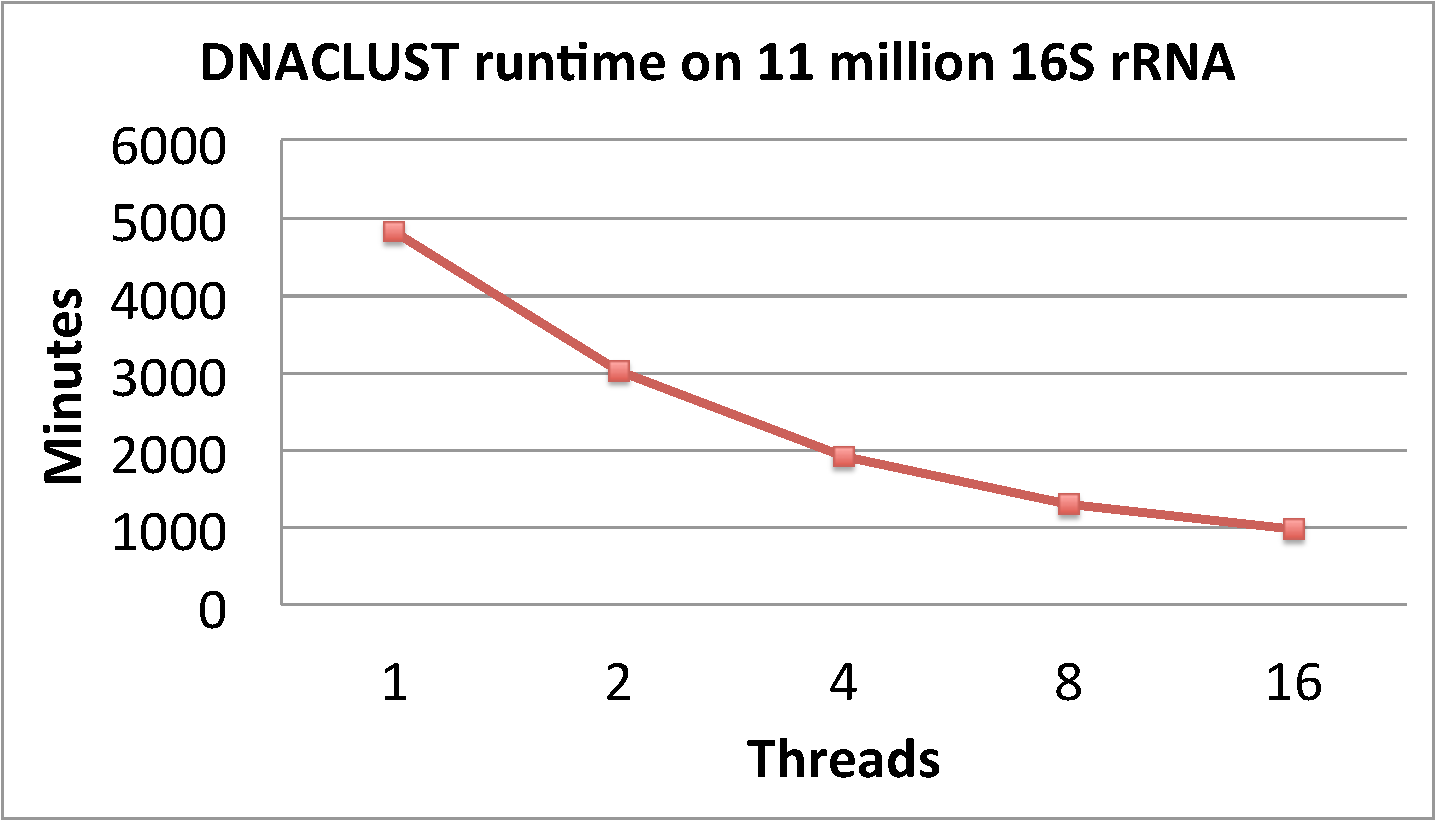
\includegraphics[width=0.5\textwidth]{parallel}
  \caption{Speedup of DNACLUST using multiple threads.}
  \label{fig:parallel}
\end{figure}

We test this parallelization using 11 million 16S rRNA (average length of 350 bps) (Figure \ref{fig:parallel}).
Going from one to two threads, and two to four threads results in a $1.6\times$ speedup.

\subsubsection{Work-based parallelization strategy}

DNACLUST keeps the database of sequences sorted to speed up the calculation of edit distance between lexicographically adjacent sequences.
Adjacent sequences that share a similar prefix allow us to reuse part of the dynamic programming table.
Evenly partitioning the sequences may split highly similar sequences into separate threads causing us to repeat work.
Instead of evenly dividing the number of sequences between threads, we can evenly divide the amount of potential work (characters we need to examine in the trie).

\begin{definition}
The {\bf trie length} is the total number of characters on the edges in the trie.
\end{definition}

Given a sorted database of sequences, we can calculate the trie length by iterating through each sequence and adding the length of the current sequence minus the longest common prefix of the current sequence and the previous sequence.
Once the trie length is calculated, we divide the trie length by the number of threads, giving us the amount of work per thread.
To actually assign sequences to threads, we repeat the above procedure, but once the current trie length exceeds the work per thread, we assign those sequences to the specific thread and set the current trie length to 0.

We compare the trie lengths of the na\"ive and work-based methods using 32 threads (Figure \ref{fig:naive_vs_work_strategy}).
Since we are only as fast as our slowest thread, in the worst case, the na\"ive method would require 12\% more work than the work-based method.
Future work involves implementing this feature into DNACLUST.

\begin{figure}[tb]
  \centering
    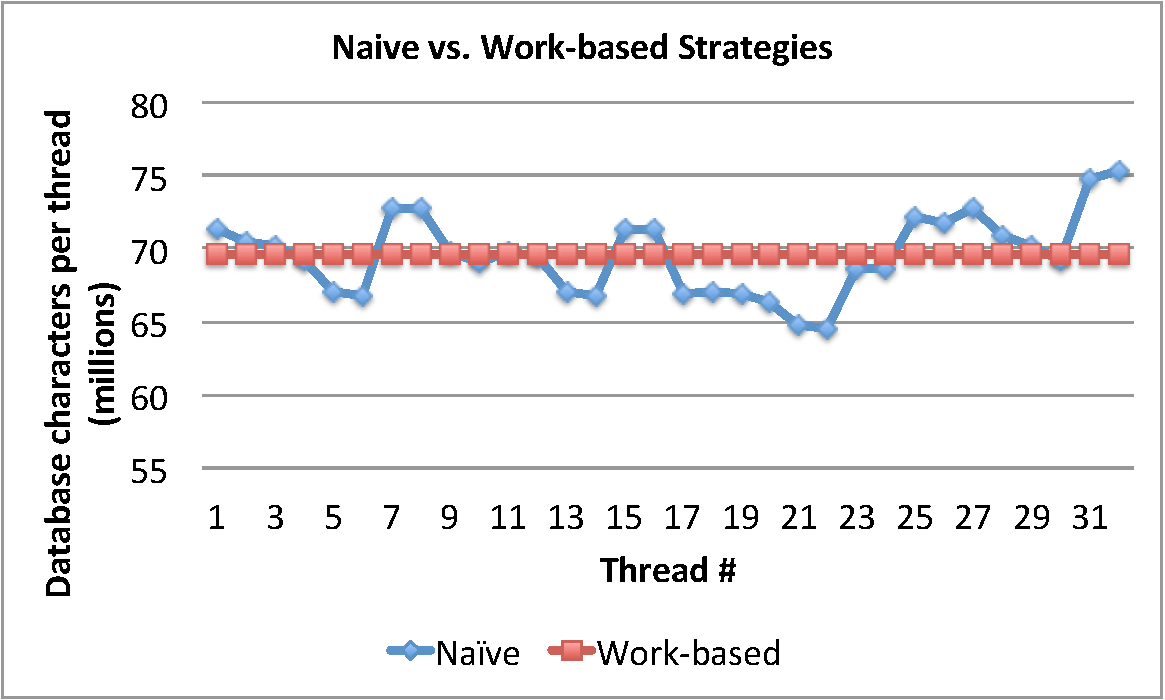
\includegraphics[width=0.5\textwidth]{naive_vs_work_strategy}
  \caption{Comparing the per-thread workload of the na\"ive and work-based parallelization methods.}
  \label{fig:naive_vs_work_strategy}
\end{figure}


\subsubsection{Parallelizing edit distance computation}

Thus far, our parallelization approaches have been focused on partitioning whole sequences.
We can parallelize the edit distance calculation since the data dependencies when updating a cell are limited.
Each cell only relies on the values stored in the horizontally, vertically, and diagonally adjacent cells.
Thus, it is possible to calculate the values along the anti-diagonals in parallel.
A group of cells can be updated in a single operation using a feature of most modern processors: SIMD instructions (single instruction multiple data).
The speedup is dependent on how many cells we can fit into the registers used for SIMD.
Results show that speedups of around six times can be achieved using modern systems\cite{farrar_striped_2007,rognes_faster_2011}.
While this speedup has a ceiling (the size of the SIMD register), the speedup will be noticeable in practice.
Our proposed work includes implementing this feature into DNACLUST's edit distance computation.

\subsection{Efficient data structures for edit distance computation}

Currently, we use an $O(nm)$ speed and time method to calculate the edit distance between two sequences of lengths $n$ and $m$ (Algorithm \ref{edit_distance}).
This cost is reduced to $O(nk)$ in the specific case of globally aligning two sequences within $k$ edits.
Globally aligning sequences may not be ideal in the case where we are aligning short WGS reads to a 16s rRNA database, which is the standard for many tools, including UCLUST.
These WGS reads are drawn randomly from the underlying genome so they can occur anywhere within the 16s rRNA gene.
Thus, we must implement a fast method to perform semi-global alignment of these sequences.

In this section, we describe how to further improve the runtime to $O(k^2)$ in the case of global alignment and $O(nk)$ for semi-global alignment using a hybrid dynamic programming method developed by Landau and Vishkin\cite{landau_introducing_1986}.

\subsubsection{Alternative representation of the dynamic programming table}

\begin{figure}[tb]
  \centering
    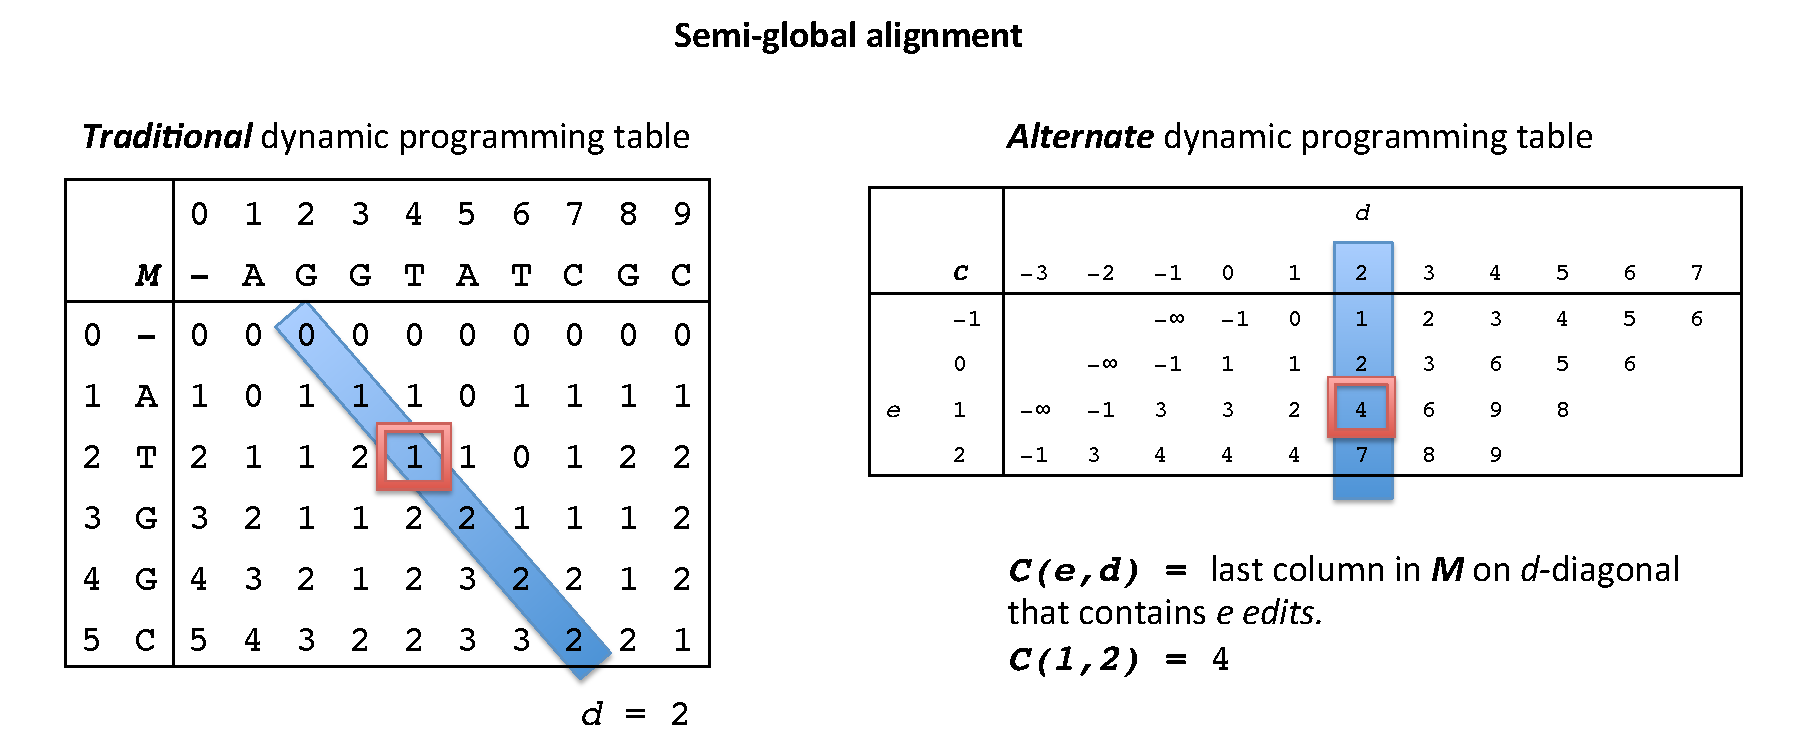
\includegraphics[width=1.0\textwidth]{alternate_table}
  \caption{Traditional and alternative dynamic programming table used to solve $k$-difference algorithm.}
  \label{fig:alternate_table}
\end{figure}
Thus far, when calculating the edit distance between sequences $t = t_1 t_2 .. t_n$ and $p = p_1 p_2 .. p_m$, cell ($i,j$) in the dynamic programming table $M$ represents the minimum edit distance between prefixes $t_{1,i}$ and $p_{1,j}$ (Algorithm \ref{edit_distance}).

\begin{definition}
Given an $n$-by-$m$ dynamic programming table, cells on a {\bf $i$-diagonal} are any cells ($z$,$j$) where $j-z=i$.
\end{definition}
%Let M be a dynamic programming table with dimensions $0 \leq m \leq n$, an {\bf $i$-diagonal} are any cells ($k$,$j$) where $j-i=k$.

\begin{definition}
A {\bf $d$-path} is a path through the dynamic programming table starting at row 0 and ending at a cell with d edits.  A d-path is {\bf farthest-reaching} in the i-diagonal if it ends in the i-diagonal and is greater than or equal to the ending column of any other d-path ending in the i-diagonal.
\end{definition}

We reduce the storage requirements by only recording the last column with $e$ edits along a given $i$-diagonal.
If we are only interested in finding alignments within $k$-difference, for each $i$-diagonal in our table, we need to record at most $O(k)$ entries.
We do not need to record more than $O(k)$ entries because in our given formulation of the problem it is impossible to decrease in the amount of edits made.
Since we only penalize start gaps in the pattern and not the text, the amount of diagonals we have to compute is $n - m + k$.
Thus, we require $O(nk)$ memory to find $k$-differences between the text and pattern.

At the high level, for every edit number $0 \leq d \leq k$, we will compute the farthest-reaching $d$-path on the $i$-diagonal using the farthest-reaching ($d-1$)-paths on diagonals $i-1$, $i$, $i+1$.
%An alternative way to view this alignment is to consider each diagonal $d$ and edit $e$ of $M$.
Let $C$ be a dynamic programming table where cell ($i,j$) now refers to the farthest-reaching column in $M$ of the $j$-diagonal that contains $i$ edits (Figure \ref{fig:alternate_table}).
For simplicity, lets assume we can access the negative $j$-diagonals of the table with cell (\_,$-j$).
Since accessing negative indexes in arrays are invalid in most programming languages, in practice we offset each diagonal by $k$.


To begin, we need to initialize the first row of $C$, where $d=0$.
A $0$-path corresponds to a path ending on the $i$-diagonal with no mismatches.
For each column $j$ ($j$-diagonal in $M$), cell $C(i,j)$ is set to the \emph{longest common extension} of $p_1..p_m$ and $t_j..t_n$.

For $d > 0$, to compute the farthest-reaching $d$-path on the $i$-diagonal, we first need to consider three different farthest-reaching ($d-1$)-paths:

\begin{itemize}
  \item {\bf ($d-1$)-path on ($i-1$)-diagonal.} We follow a horizontal edge (a space in $p$), which increases the column index by 1.
  \item {\bf ($d-1$)-path on ($i$)-diagonal.} We follow an edge corresponding to a mismatch between a character of $p$ and $t$ and increment the column index by 1.
  \item {\bf ($d-1$)-path on ($i+1$)-diagonal.} We follow a vertical edge (a space in $t$).  We do not increment the column index in this case.
\end{itemize}

Once we have the largest column index ($col$) of a ($d-1$)-path, then we find the longest common extension starting from $t_{col}$ and $p_{col-d}$.
An acceptable alignment will be any cell $C(e,d)$ whose value is greater than $m + d$.
This means that the full pattern has been matched in $\leq k$ edits.


 \begin{algorithm}
 \caption{Landau-Vishkin $k$-differences algorithm. $O(kn)$ work.}\label{landau_vishkin}
 \begin{algorithmic}[1]
 \Procedure{ComputeKDifferences}{$t,p,k$}
 \State $n\gets |t|$
 \State $m\gets |p|$

 \For{$d=0 .. n - m + k + 1$}  \State $C(-1,d) \gets i$ \EndFor \Comment Set first row of table $C$ to one minus its diagonal. 
 \For{$d= -(k+1) .. -1 $}
    \State $C(|d| - 1 ,d) \gets -1$
    \State $C(|d| - 2 ,d) \gets -\inf$
\EndFor

 \For{$i=0 .. n-m+k$} \Comment Process table along the anti-diagonals.
 \For{$e=0 .. k$}
  \State $d \gets c - e$
  \State $col \gets max(C(e-1,d-1) + 1,C(e-1,d)+ 1,C(e-1,d+1))$
  \While{$col < n$ \textbf{and} $col - d < m$ \textbf{and} $x_{col+1} == y_{col+1-d}$}
    \State $col \gets col + 1$
  \EndWhile
  \State $C(i,j) \gets \text{min}(col, m + d, n)$
  \If {$C(i,j) \geq m + d$} 
  \Return $\text{Occurrence found}$
  \EndIf
\EndFor
\EndFor
\Return $\text{No occurrence found}"$
\EndProcedure
\end{algorithmic}
\end{algorithm}

There are two ways we can calculate the cells of $C$.
Cell $C(i,j)$ relies on the values in adjacent cells: $C(i-1,j-1)$, $C(i-1,j)$, and $C(i-1,j+1)$
Once we initialize the first row of $C$, we can proceed row-by-row.
However, in the next section, we will describe why we populate the cells an anti-diagonal at a time (Algorithm 2).

For each edit ($0\leq e \leq k$) and diagonal ($-k \leq d \leq n-m$), we need to record the longest reaching $d$-path, so the amount of memory required is $O(nk)$.
Finding the longest common extension between two substrings in $p$ and $t$ requires $O(n)$ time.
However, we can use a suffix tree to store our center ($t$) and reduce the longest common extension time down to $O(1)$ time\cite{gusfield_algorithms_1997}, reducing the overall runtime down to $O(kn)$.

\begin{comment}
\begin{equation}
\begin{aligned}
\text{col} & = \quad max
\begin{cases}
\quad C[i - 1, j-1] + 1 \\
\quad C[i - 1, j] + 1 \\
\quad C[i - 1, j+1] 
\end{cases} \\
C[i, j] & =  \quad \text{col} + \text{LCE}[t_{\text{col}}, p_{\text{col} - \text{j}}]
\end{aligned}
\end{equation}
\end{comment}





%-Compare the two approaches in terms of cells of the dp matrix that need to be computed.

\subsubsection{Efficient $k$-difference implementation}
%Although our implementation of Landau-Vishkin does not provide a constant time
We provide an implementation of both the n\"aive and the Landau-Vishkin algorithms written in C.
For our experiment, we created a 1,000 sequence sample from an environmental 16S rRNA data set.
The database sequences ranged in length from 300bps to 600bps.
We randomly selected a sequence from the database to serve as our center. 
The center was aligned against the database sequences with $k=5$ using both methods (Table \ref{table:naive_vishkin}).
Runtimes were averaged over 100 runs.

It is important to note that in our current implementation we used an inefficient method for computing the longest common extension between two substrings.
Despite this, our implementation of the Landau-Vishkin algorithm is \emph{25x} faster than the na\"ive method.



\begin{center}
\begin{table}[tb]
\centering
\begin{tabular}{c|c}
               & Semi-global (k=5) \\
\hline 
Na\"ive          & 1.022 sec  \\
Landau-Vishkin & 0.040 sec \\
\hline 
Speedup        & 25.599x
\end{tabular}
\caption{Runtime comparison of the na\"ive and Landau-Vishkin\cite{landau_introducing_1986} methods for finding all semi-global alignments within $k$-differences. The center (a 637bp sequence) was aligned against a database consisting of 1,000 16S rRNA sequences (ranging in lengths from 300-600bp) with $k=5$.  Runtimes were averaged over 100 runs.}
\label{table:naive_vishkin}
\end{table}
\end{center}


\subsubsection{Exploiting a sorted sequence database}
DNACLUST leverages the fact that the database of sequences are highly similar.
By sorting the database sequences, we can reuse the first $l$ rows of the dynamic programming table between database sequences $i$ and $i+1$, where $l$ is equal to the longest common prefix of $i$ and $i+1$.
Our current implementation does not account for this; however, here we will outline the steps necessary to recreate this feature with our alternative dynamic programming table implementation.

In the traditional dynamic programming table, the $i$-th row of the table correspond to the $i$-th character of the pattern and the $j$-th column corresponds to the $j$-th character of the text.
After populating the full dynamic table, we now attempt to align the new pattern with the text.
The new pattern shares $l$ characters with the previously aligned pattern.
Here we can start aligning from the $(l+1)$-th row because we have already aligned the prefix ending at position $l$ of the new pattern with the previous pattern.


\begin{figure}[tb]
  \centering
    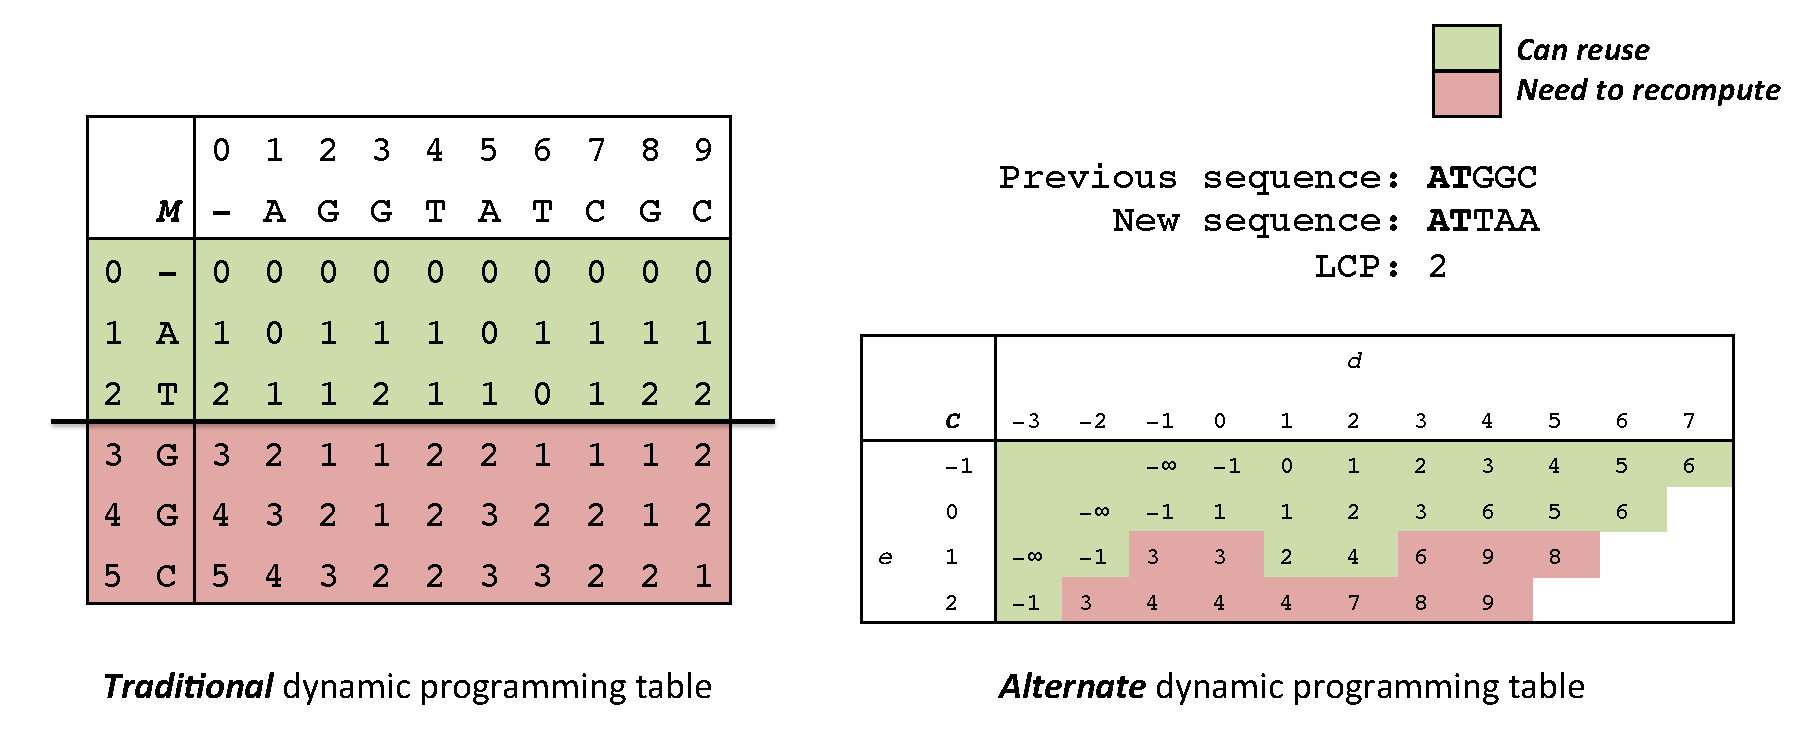
\includegraphics[width=1.0\textwidth]{work_saving}
  \caption{Exploiting sorted sequence database to speedup $k$-difference algorithm.}
  \label{fig:work_saving}
\end{figure}


In our alternative dynamic programming table, the $i$-th row of the table corresponds to the $i$-th allowed edit distance and the $j$-th column corresponds to the $j$-th diagonal of the traditional dynamic programming table.
It becomes trickier to reuse information from this dynamic programming table because edits along a given diagonal in the traditional dynamic programming table may start before the $i$-th row and extend past the $(l+1)$-th row (Figure \ref{fig:work_saving}).
%Thus, for each diagonal we need to find all acceptable cells within 
We can only reuse the information in this alternative dynamic program table if along a given $i$-diagonal and edit distance, the farthest-reaching column ends on or before the $(i+l)$-th column.

In Algorithm \ref{landau_vishkin}, we calculated the cells in table $C$ starting from the 0 anti-diagonal.  Cell $C(e,d)$ lies on the $(e+d)$ anti-diagonal.
When calculating $C(e,d)$, we first find the farthest-reaching column (max of $C(e-1,d-1) + 1$, $C(e-1,d)$ + 1, $C(e-1,d-1)$) then extend the match between the pattern and text as far as possible.
As we proceed downwards along the given $c$ anti-diagonal, if the value in the cell $C(e,d) - d$ is greater than the $l$ we need to recalculate the cell.
We subtract by $d$ to correct for the offset start position of the $d$-diagonal.
A value greater than $l$ indicates that the longest $e$-path on the $d$-diagonal extends past the shared prefix of the current and previous patterns.
Thus, for a given $e$ and $d$, if $C(e,d) - d > l$, we need to recalculate the cell.
If we have to recalculate $C(e,d)$ then we are forced to recalculate any cells that directly depend on $C(e,d)$, which in this case would be $C(e+1, d-1)$, $C(e+1, d)$, and $C(e+1, d+1)$.

One important thing to note is that if $C(e,d)$ is the first cell in column $d$ that we have to recompute, then we can save this index to speed up finding the first cell to recompute in column $d+1$.
Assume $C(e,d)$ does \emph{not} need to be recomputed.
That means that the value (farthest-reaching column) in cells $C(e-1,d-1)$, $C(e-1,d)$, and $C(e-1,d+1)$ are all less than $C(e,d)$ and do not need to be recomputed.
If any of the three adjacent cells above $C(e,d)$ had to be recomputed, then we would be forced to recompute $C(e,d)$.

\begin{theorem}
%For a given $d$, let $j$ be the lowest $e$ such that $C(j,d)$ does not need to be recomputed and $C(j+1,d)$ has to be recomputed.  The largest $e$ that does not need to be recomputed in column $d+1$ is either $j-1$, $j$, or $j+1$.
For a given $d$, let $j$ be the lowest row index ($0 \leq j \leq k$) such that $C(j,d)$ needs to be recomputed, but $C(j-1,d)$ does not need to be recomputed. The lowest row index that needs to be recomputed in column $d+1$ is either $j-1$, $j$, or $j+1$.
\end{theorem}

\begin{proof}
Assume not and $j-2$ is the lowest row index that needs to be recomputed in column $d+1$.  If $C(j,d)$ is the lowest row index in $d$ that needs to be recomputed, then $C(j-1,d)$ does not need to be recomputed.  If $C(j-2,d+1)$ needs to be recomputed, then $C(j-1,d)$ needs to be recomputed as well since $C(j-1,d)$ depends on $C(j-2,d-1)$, $C(j-2,d)$, $C(j-2,d+1)$.  However, we have already said that $j$ is the lowest row index such that $C(j-1,d)$ does not need to be recomputed, resulting in a contradiction.  A similar reasoning can be done when for $j-3$, $j-4$, ..., 0.
%, and since $C(j,d)$ depends on cells $C(j-1,d-1)$, $C(j-1,d)$, and $C(j-1,d-1)$, $C(j-1,d)$ does \emph{not} to be recomputed.  

Now assume $j+2$ is the lowest row index that needs to be recomputed in column $d+1$, making $j+1$ the last row index that does not need to be recomputed.  If $C(j+1,d+1$) does need to be recomputed, then the cells it depends on ($C(j,d)$, $C(j,d+1)$, $C(j,d+2)$) do not need to be recomputed.  However, we have already said that $j$ is the lowest row index such that $C(j,d)$ needs to be recomputed.  Hence, another contradiction.  A similar strategy can be used for $j+3$, $j+4$ ..., $k$.

%  If $C(j+2,d+1)$ is the lowest cell in column $d+1$ that needs to be recomputed, then by definition $C(j+1,d+1)$ does not need to be recomputed.

\end{proof}

The runtime of finding the starting cells to recompute along on an anti-diagonal takes $O(k)$ work because we start on the first anti-diagonal and proceed downwards until we find the first the cell where $C(e,d) - d > l$.
Then when processing the next anti-diagonal, we only need to look at potentially three start positions of the first cell in that column to be recomputed (constant work), taking only $O(k)$ time to find the starting point for recomputing the cells of $c$.  Since the columns are increasing down the anti-diagonal, it would also be possible to perform a binary search to find the appropriate start location, reducing the time to $O(lg(k))$.
However, since the values of $k$ are often very small in practice, little practical benefit would be obtained.

%The steps outlined above will allow for us to to perform efficient semi-global alignment.

%In the true implementation of it requires only $O(1)$ work to calculate the longest common extension between substrings starting at $t_i$ and $p_j$.
%Asymptotically, it requires no more work to recompute $C(e,d)$.
%Since our current implementation does not have this feature yet, we expect that

%\subsubsection{Suffix tree cluster center representation}

\subsection{Handling ambiguous reads}

Often, a goal of metagenomic studies is to compare the microbial composition across multiple samples and conditions.
Qin et al. looked for gut microbial markers that might be useful for classifying type 2 diabetes\cite{qin_metagenome-wide_2012}.
Before we can detect differential abundance across samples, the sample sequences have to be clustered into OTUs, counted, and then normalized\cite{paulson_differential_2013}.
Thus far in this prospectus, we have discussed methods for speeding up the alignment of sequences to a center, but we have yet to discuss how to handle ambiguous reads.

When a sequence is being recruited by a center, it is possible that this sequence is within some distance from another potential center.
Henceforth, we refer to a sequence that lies within a given distance from multiple centers as \emph{ambiguous}.
Currently in DNACLUST, UCLUST, and CD-HIT, an ambiguous sequence is recruited by the first center that it encounters.
Depending on the number of ambiguous of sequences, this may affect the resulting cluster abundances.
For example, if we are clustering short WGS reads using a database of 16S rRNA genes, the first 16s rRNA gene we select as a center will preferentially recruit all of the WGS reads that happen to fall within a conserved region of the gene.
This could drastically affect downstream analyses for detecting differentially abundant OTUs.

\begin{table}[t]
\centering
\begin{tabular}{@{}ll@{}}
\toprule
Strategy   & Clusters  \\ \midrule
Unique     & 3,031,761 \\
Ambiguous  & 5,085,988 \\
Ones       & 6,201,399 \\
Random     & 5,183,737 \\
Proportion & 6,201,399 \\ \bottomrule
\end{tabular}
\caption{Comparing the total number of gene clusters found using the different strategies for aligning ambiguous reads on the Qin et al. type 2 diabetes data set.}
\label{table:ambiguous_reads}
\end{table}

Here, we describe different methods for assigning ambiguous reads and constructing the count matrix, where the rows represent different OTUs, the columns represent different samples, and the cell $(i,j)$ corresponds to the count of OTU $i$ in sample $j$.
% on analyzing these count matrices (such as detecting differentially abundant OTUs) could lead to incorrect results.

In DNACLUST, we mark any sequence \emph{black} that has been assigned to a cluster center, which signifies that the sequence will not be aligned to another center nor chosen as a potential center.
We have added the option DNACLUST to print an inverted index mapping sequences to their potential centers.
We accomplish this by marking a sequence \emph{gray} when it is aligned to a cluster center, which signifies that the sequence \emph{can} be aligned to other centers, but it cannot be chosen as a potential center.
This inverted index allows users the option to their preferred method for assigning ambiguous reads.

The first method is to simply discard any ambiguous reads and only consider reads that can be uniquely aligned to a single center.
One potential issue with this approach is when comparing the abundances of OTUs \emph{within} a sample.
Two OTUs with equal abundance, but an unequal number of unique regions, will not be equal in the count matrix.
This problem can also occur across samples, where one sample contains the two OTUs, and the other sample only contains one of the OUTs.
If in reality the shared OTU occurs at the same relative abundance across samples, we may erroneously find an increased abundance in the second sample if we only look at uniquely aligned reads.

Another way to assign ambiguous reads is to randomly assign them to the set of potential centers.
An issue with this approach is that we may assign reads to an OTU that does not exist within our sample, the read just happens to align to a conserved region present across multiple OTUs.

Similarly, instead of randomly assigning the reads, we can assign a fractional count to each center.  Although, with a large number of ambiguous reads, the fractional counts should be close to the previous randomly assign approach.

Lastly, we can assign a read based on the proportion of uniquely aligned reads to the center.  In other words, if a read can align equally well to two different centers, but one center contains uniquely aligned reads and the other contains none, then it is more probable that the read came from the first center.  This approach should better handle the potential false OTU detection present with random and fractional assignment of reads.
We add a small pseudocount of one to each OTU to help in the case of low coverage or the possibility that the OTU contains no unique regions.
An issue with this current approach, however, is that we do not normalized by the possibility of repeats within the center.
A more intelligent approach is to use a maximum likelihood method to assign the ambiguous reads with the added constraint being coverage across the center should be uniform\cite{patro2013sailfish}.

For our proposed work, we want to reanalyze these large publicly available data sets (such as Qin et al's type 2 diabetes data set \cite{qin_metagenome-wide_2012}) and see if there claims still hold depending on their read mapping strategy.
As a preliminary experiment, we aligned the reads using Bowtie2 (a fast read alignment tool)\cite{langmead2012fast} to the Human Microbiome Project's gene clusters (\url{http://hmpdacc.org/HMGC/}) using the different read strategies (Table \ref{table:ambiguous_reads}).
One important thing to note is that when we only count gene clusters that have at least one unique read mapping to it we had nearly 50\% less gene clusters than if we randomly assigned ambiguous reads.
Since these high profile studies are drawing conclusions from these count matrices, more week needs to be done observing the effect of ambiguous read alignments. 
